\documentclass[11pt]{beamer}
\usepackage[UTF8,scheme=plain]{ctex}
\usepackage{listings}
\usepackage[utf8]{inputenc}
\usepackage[T1]{fontenc}
\usepackage{amsmath}
\usepackage{amsfonts}
\usepackage{amssymb}
\usepackage{graphicx}
\usetheme{Boadilla}

\usepackage{framed} % 可以用 \begin{shaded},即背景色块
\definecolor{shadecolor}{rgb}{0.9,0.9,0.9}

\newcommand{\kong}[1][0.5]{\vspace{#1cm}}

\begin{document}
	\author{ 路毅 \hspace{0.3cm} 曲阜师范大学 }
	\date{\number\year 年 \number\month 月 \number\day 日}
	\title{数学物理方法第七章}

\begin{frame}
	\maketitle
\end{frame}

\kaishu

\begin{frame}{第七章:一维波动方程的傅里叶解}
\begin{itemize}
	\item 第一节:一维弦振动方程
	\vspace{1cm}
	\item 第二节:傅里叶解及其物理意义
\end{itemize}
\end{frame}

\begin{frame}{软绳小振动方程}

\kong[1]
软:没有法向应力,只有切向张力。

\kong[1]
小振动:振动幅度不大,绳上每个质点偏离平衡位置的幅度都较小。
\end{frame}

\begin{frame}{软绳小振动方程}
\begin{figure}
\centering
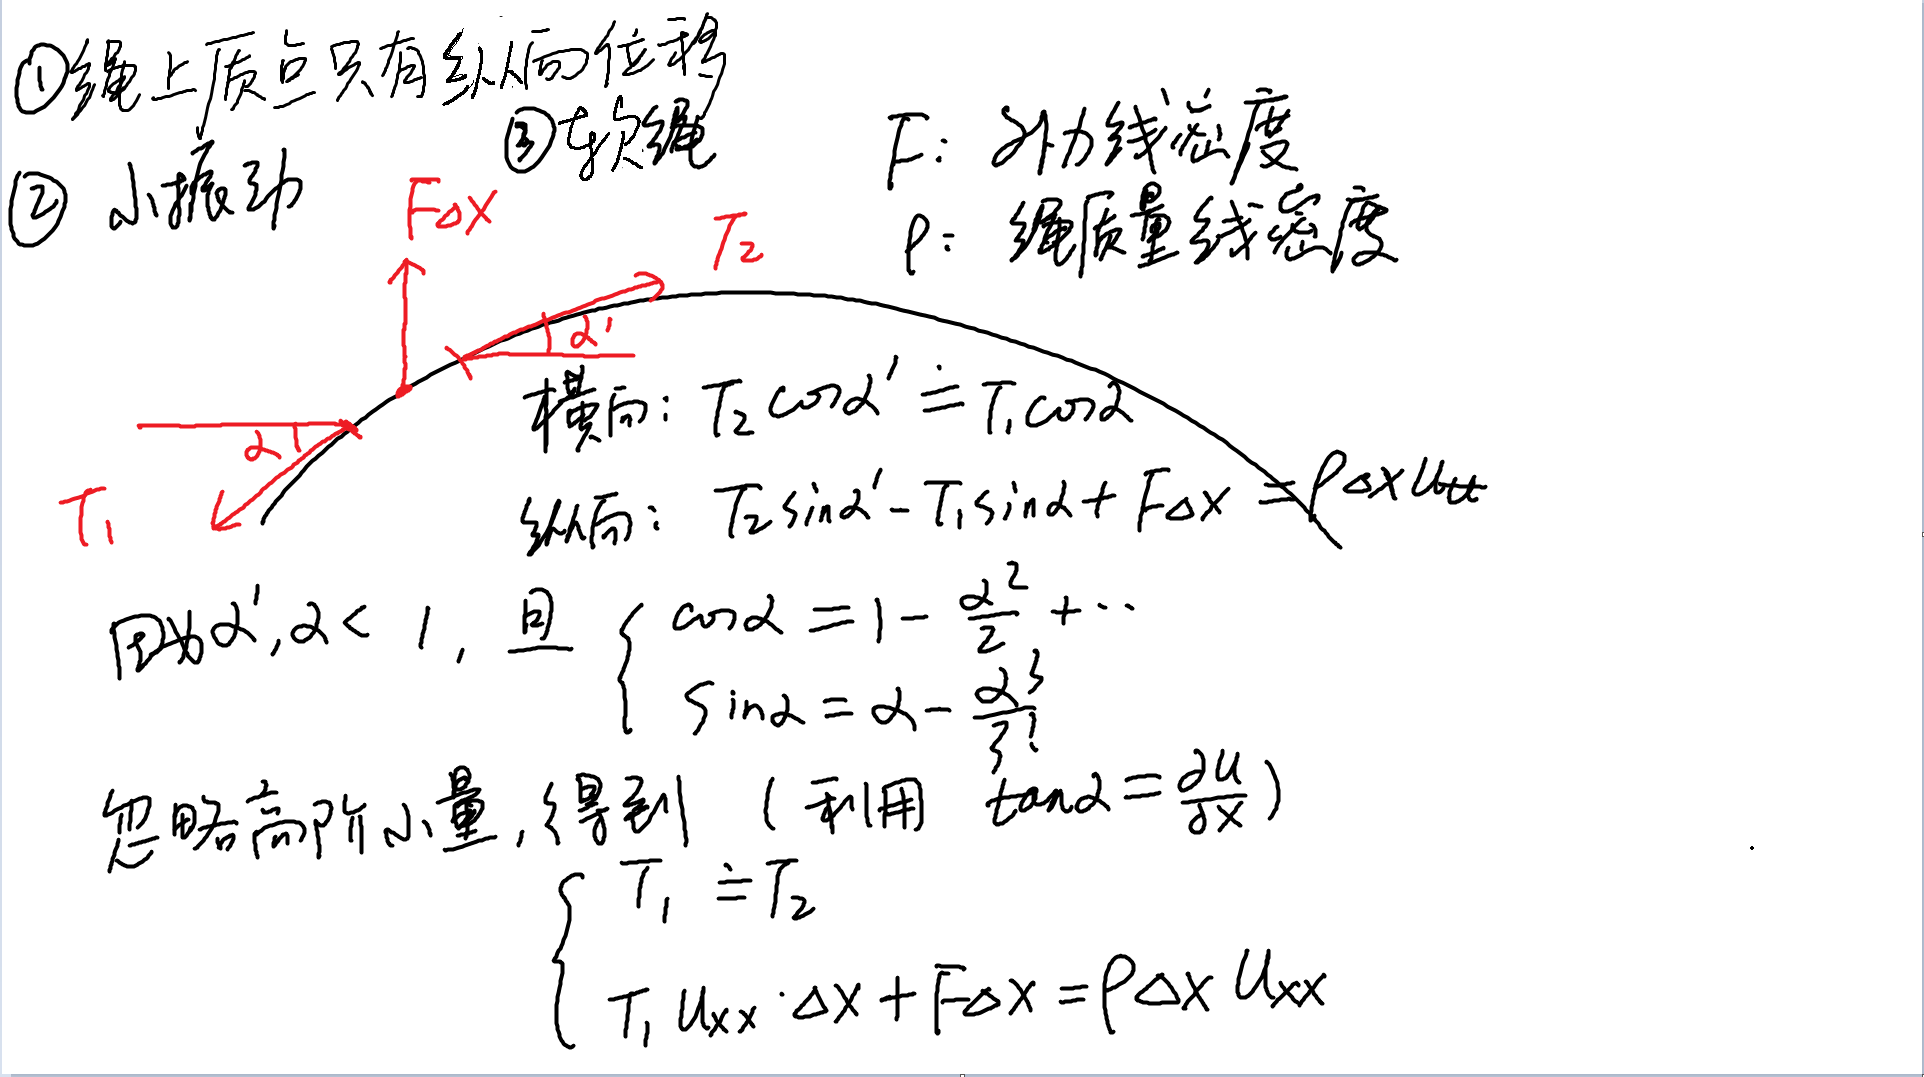
\includegraphics[width=\linewidth]{弦振动方程}
\end{figure}
其中,$u_{xx}$表示对$x$二阶偏导数,$u_{tt}$表示对$t$二阶偏导数。
\end{frame}

\begin{frame}{振动方程}
取$ a^2 = T/\rho, f = F/\rho$,则有
\begin{equation}
u_{tt} = a^2 u_{xx} + f.
\end{equation}
如果没有外力,即弦自由振动,则有
\begin{equation}
u_{tt} = a^2 u_{xx}.
\end{equation}
\end{frame}

\begin{frame}{边界条件、初始条件}
边界条件:$u(0,t), u(l,t)$。
\begin{itemize}
\item $u(0,t)=\mu(t)$,狄利克雷边界条件。
\item $u_x(0,t) = \nu(t)$,诺依曼边界条件。
\item $u_x(0,t) - hu(0,t) = \theta(t)$,罗宾边界条件。
\end{itemize}

\kong[0.5]
初始条件:$u(x,0),u_t(x,0)$,即初始时刻绳的形状,各个质点的速度。
\end{frame}

\begin{frame}{两端固定、自由振动}
\begin{eqnarray}
u_{tt} =& a^2 u_{x}, &\text{齐次} \\
 u(0,t) =& u(l,t) = 0, &\text{两端固定}\\
 u(x,0) =& \varphi(x), u_t(x,0) = \psi(x), &\text{初始位置、速度}
\end{eqnarray}
我们先抛开初始条件,只管边界条件,得到通解形式,再用初始条件约束通解,得到特解。
\end{frame}

\begin{frame}{分离变量法}
假设
\begin{equation}
u(x,t) = X(x) T(t),
\end{equation}
带入自由振动方程,则有
\begin{equation}
a^2 X''/X = T''/T,
\end{equation}
方程左边只与$x$有关,右边只与$t$有关,左右两边的值在任意$x,t$都是一个常数,假设这个常数是$- \lambda$。
\end{frame}

\begin{frame}{两端固定:通解}
根据边界条件$u(0,t)=u(l,t)=0$,得到$ X(0) = X(l) =0$。
\begin{equation}
X'' + \lambda X = 0.
\end{equation}
1. 若$\lambda=0$,则有$X(x) = C_1 x + C2$,带入边界条件得到$X(x)=0$。

2. 若$\lambda<0$,则有
\begin{equation}
X(x) = A e^{\sqrt{-\lambda}x} + B e^{-\sqrt{-\lambda}x},
\end{equation}
代入边界条件$u(0,t)=u(l,t)=0$,得到$ X(0) = X(l) =0$,所以有
\begin{eqnarray}
A + B = 0, \\
A e^{\sqrt{-\lambda}l} + B e^{-\sqrt{-\lambda}l} = 0.
\end{eqnarray} 
得到$ A=B=0$,即$X(t)=0$。
\end{frame}

\begin{frame}{两端固定:通解}
3. 若$\lambda>0$,则有
\begin{equation}
X(x) = A \cos(\sqrt{\lambda}x) + B \sin(\sqrt{\lambda}x) ,
\end{equation}
代入$ X(0) = X(l) =0$,得到
\begin{eqnarray}
A = 0, \\
B \sin(\sqrt{\lambda}l)= 0.
\end{eqnarray} 
得到$A=B=0$(平庸解),或
\begin{eqnarray}
B \neq 0, \\
\sin( \sqrt{\lambda} l) = 0 \Rightarrow \sqrt{\lambda} = n \pi / l, n \in Z^+.
\end{eqnarray}
所以非平庸解为$B\neq 0$,
\begin{equation}
X_n(x) = B_n \sin( n\pi x /l), ~~ n=1,2,\cdots
\end{equation}
相应地
\begin{equation}
T_n(t) = C^\prime_n \cos(n\pi a t/l) + D^\prime_n \sin(n\pi a t/l).
\end{equation}
\end{frame}

\begin{frame}{两端固定:通解}
所以$u(x,t)$在特定$n$值的解为
\begin{equation}
u_n(x,t) = C_n \sin(n\pi x /l) \cos(n\pi a t/l)
			+ D_n \sin(n\pi x/l) \sin(n\pi at/l).
\end{equation}
$u(x,t)$的通解为
\begin{eqnarray}
u(x,t) &=& \sum^\infty_{n=1}u_n(x,t) \\
		&=& \sum^\infty_{n=1} C_n \sin(n\pi x /l) \cos(n\pi a t/l) + \sum^\infty_{n=1} D_n \sin(n\pi x/l) \sin(n\pi at/l). \nonumber
\end{eqnarray}
\end{frame}

\begin{frame}{带入初始条件}
带入初始条件得到
\begin{eqnarray}
u(x,0) = \sum^\infty_{n=1} C_n \sin(n\pi x/l) = \varphi(x), \\
u_t(x,0) = \sum^\infty_{n=1} Dn \sin(n\pi x/l) (n\pi a/l) = \psi(x).
\end{eqnarray}
利用 $\int^l_{0} \sin(n\pi x/l) \sin(m\pi x/l) dx = \delta_{mn} \frac{l}{2}$,可以解出 $C_n, D_n$的值,
\begin{eqnarray}
C_n &=& \frac{2}{l} \int^l_0 \varphi(x) \sin(n\pi x/l) dx, \\
D_n &=& \frac{2}{n\pi a} \int^l_0 \psi(x) \sin(n\pi x/l) dx.
\end{eqnarray}
\end{frame}

\begin{frame}{傅里叶级数收敛性}
狄利克雷收敛条件:绝对可积,任一有限区间只能取有限个最值,任何区间只有有限个第一类间断点。

\kong[1]
物理问题中$\varphi(x), \psi(x)$都是满足上述条件的函数,所以如上求出$C_n,D_n$以后代入
\begin{eqnarray}
u(x,0) = \sum^\infty_{n=1} C_n \sin(n\pi x/l), \\
u_t(x,0) = \sum^\infty_{n=1} Dn \sin(n\pi x/l) (n\pi a/l).
\end{eqnarray}
$u(x,0), u_t(x,0)$一定会收敛至$\varphi(x), \psi(x)$。
\end{frame}

\begin{frame}{物理阐释}
\begin{itemize}
\item 对任意正整数$n$
\begin{equation}
C_n sin(n\pi x/l)\cos (n\pi at/l) + D_n \sin(n\pi x/l) \sin( n\pi at/l),
\end{equation}
通过三角函数和角公式可以写作
\begin{eqnarray}
&& E_n \sin( n\pi x/l ) \sin( n\pi at/l - \delta)  \\
&& = \frac{E_n}{2}\cos( n\pi (x-at)/l + \delta )
- \frac{E_n}{2}\cos( n\pi (x+at)/l - \delta ).\nonumber
\end{eqnarray}
这是两列振幅相同的行波,一列向左传播,一列向右传播,波速均为$a$, 角频率均为$\omega_n = n\pi a/l$,干涉形成驻波,$x=0,x=l$是两个波节(振动为0的点)。
\end{itemize}
\end{frame}

\begin{frame}{物理阐释}
\begin{itemize}
\item 两端固定的绳波由无数个这样的简谐驻波性叠加合成,振幅、相位由初始时位移、速度分布决定。
\item 任意时刻,绳子的状态由所有简谐分波叠加得到。
\item 对于弦乐器(钢琴、吉他、尤克里里、小提琴),弦振动时,同时有角频率$\omega_1, \omega_2, \cdots$的音,基频$\omega_1$的振幅一般最大,$\omega_2, \cdots$的音叫做泛音,不同乐器的泛音组合系数不同,构成不同的音色。
\item 课程论文参考题目——{\bf 解码乐器的音色}:学习快速傅里叶变换(FFT)算法,编写一个小程序,尝试处理不同乐器的声音音轨文件,进行傅里叶分解,做出泛音系数曲线,进行对比。
\end{itemize}
\end{frame}

\begin{frame}{作业}
习题 1,3,5
\end{frame}

\end{document}

